\chapter{Current state of the project}\label{ch:state}

\section{Planning}
\subsection{What have we done ?}
The first semester of the academic year 2021 was meant to research and become comfortable with new tools according to our planning. We had to research how to implement such an IoT Network and how sound must be captured. 

\begin{figure}[hb]\centering
     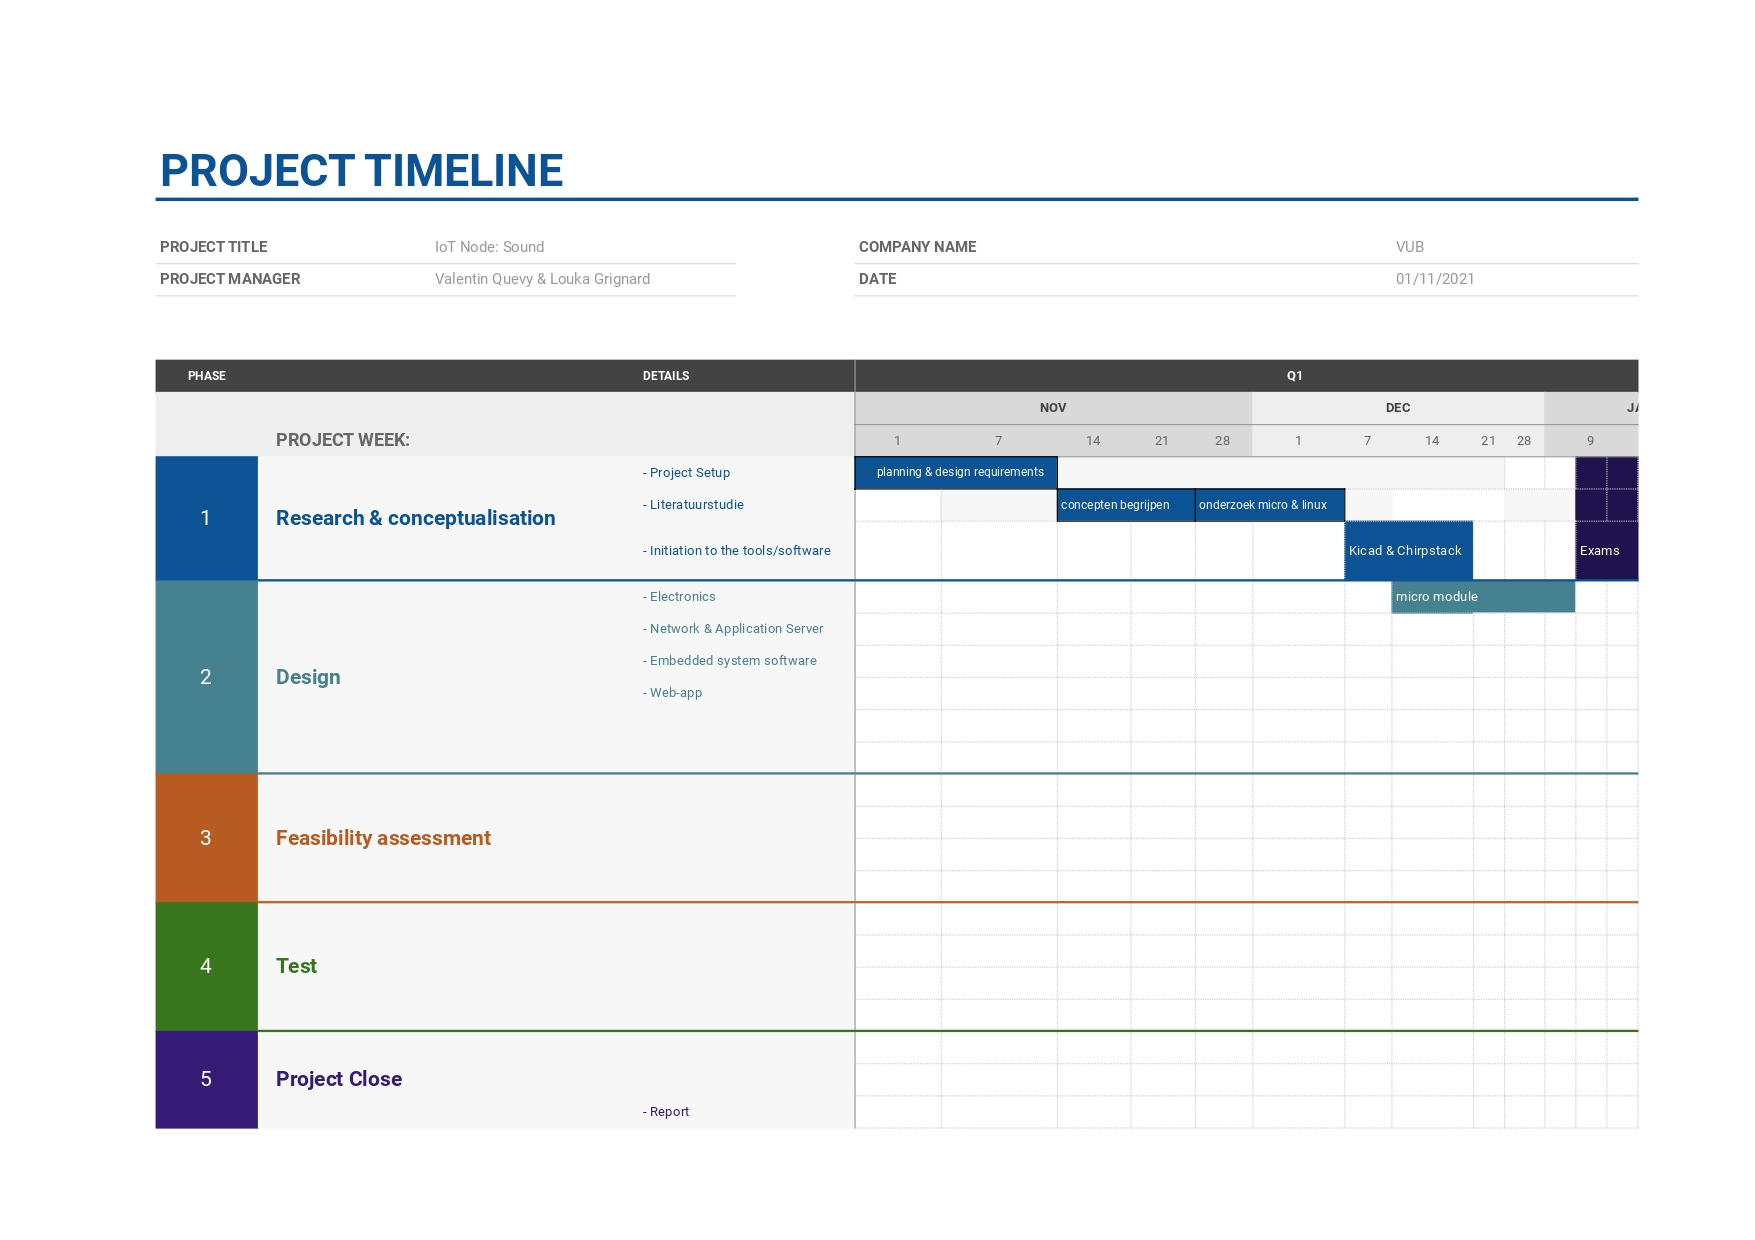
\includegraphics[width=1\textwidth,height=1\textheight,keepaspectratio]{figs/timeline.jpg}
	\caption{Project timeline}\label{fig:planning}
\end{figure}

During the research we discovered new tools like Kicad \& Chirpstack and learned using them.
For the hardware part we designed our micro-module, we still have to purchase the micro and print the pcb.

For the server part we had to learn more about the LoRa communication technology before implementing a gateway. The next step would be to try sending information via our gateway to the Network server.

\subsection{What are the next steps ?}

We followed the planning for the most part in terms of research. We still have to print our pcb of our micro-module before testing \& calibrating it with a wave-generator.
For the server part we received the needed material mid-december. We will have to test our gate-way \& server connection with chirp stack in order to implement nodes in the network.

In order to finish this project during the first sitting we will have a big workload during the second semester. The minimum for finishing this project would be to have at least one node communicating the sound measurements to our gateaway and displaying it on a web-site. We estimate a rate of succes of 65\% for finishing this project on time.

The next steps we will take are mentioned in the \href{https://docs.google.com/spreadsheets/d/1MnJvkWRLTGnZnVPzwmWV14atqugAE_Fr8enjzExGkms/edit?usp=sharing}{planning} : design, feasibility assesment, test and project close.

During february-march we are going to create the Network server with chirpstack on a Virtual Machine running Linux with Ubuntu as distribution. The micro-module will be printed and tested with our pycom microcontroller board. Then we will program our microcontroller to calculate the Fast Fourrier Transform of the signal and send it via LoRa to our gateaway.


The next deadlines are:
\begin{itemize}
  \item[\ding{43}] micro module printed \& tested - mid February
  \item[\ding{43}] setup chirpstack server network - mid February
  \item[\ding{43}] gateaway connection to server network - end February 
  \item[\ding{43}] python script for sound measurement - mid March
  \item[\ding{43}] node implementation in the network - end March
  \item[\ding{43}] node shield (battery, antenna, micro) - end March
  \item[\ding{43}] website draft - begin April
\end{itemize}

If we spend enough time and collect the needed material on time we will be able to meet the deadlines. We still have to purchase the \href{https://www.digikey.be/en/products/detail/pui-audio-inc/DMM-4026-B-I2S-R/11587483}{MEMS-micro}.

\begin{figure}[hb]\centering
     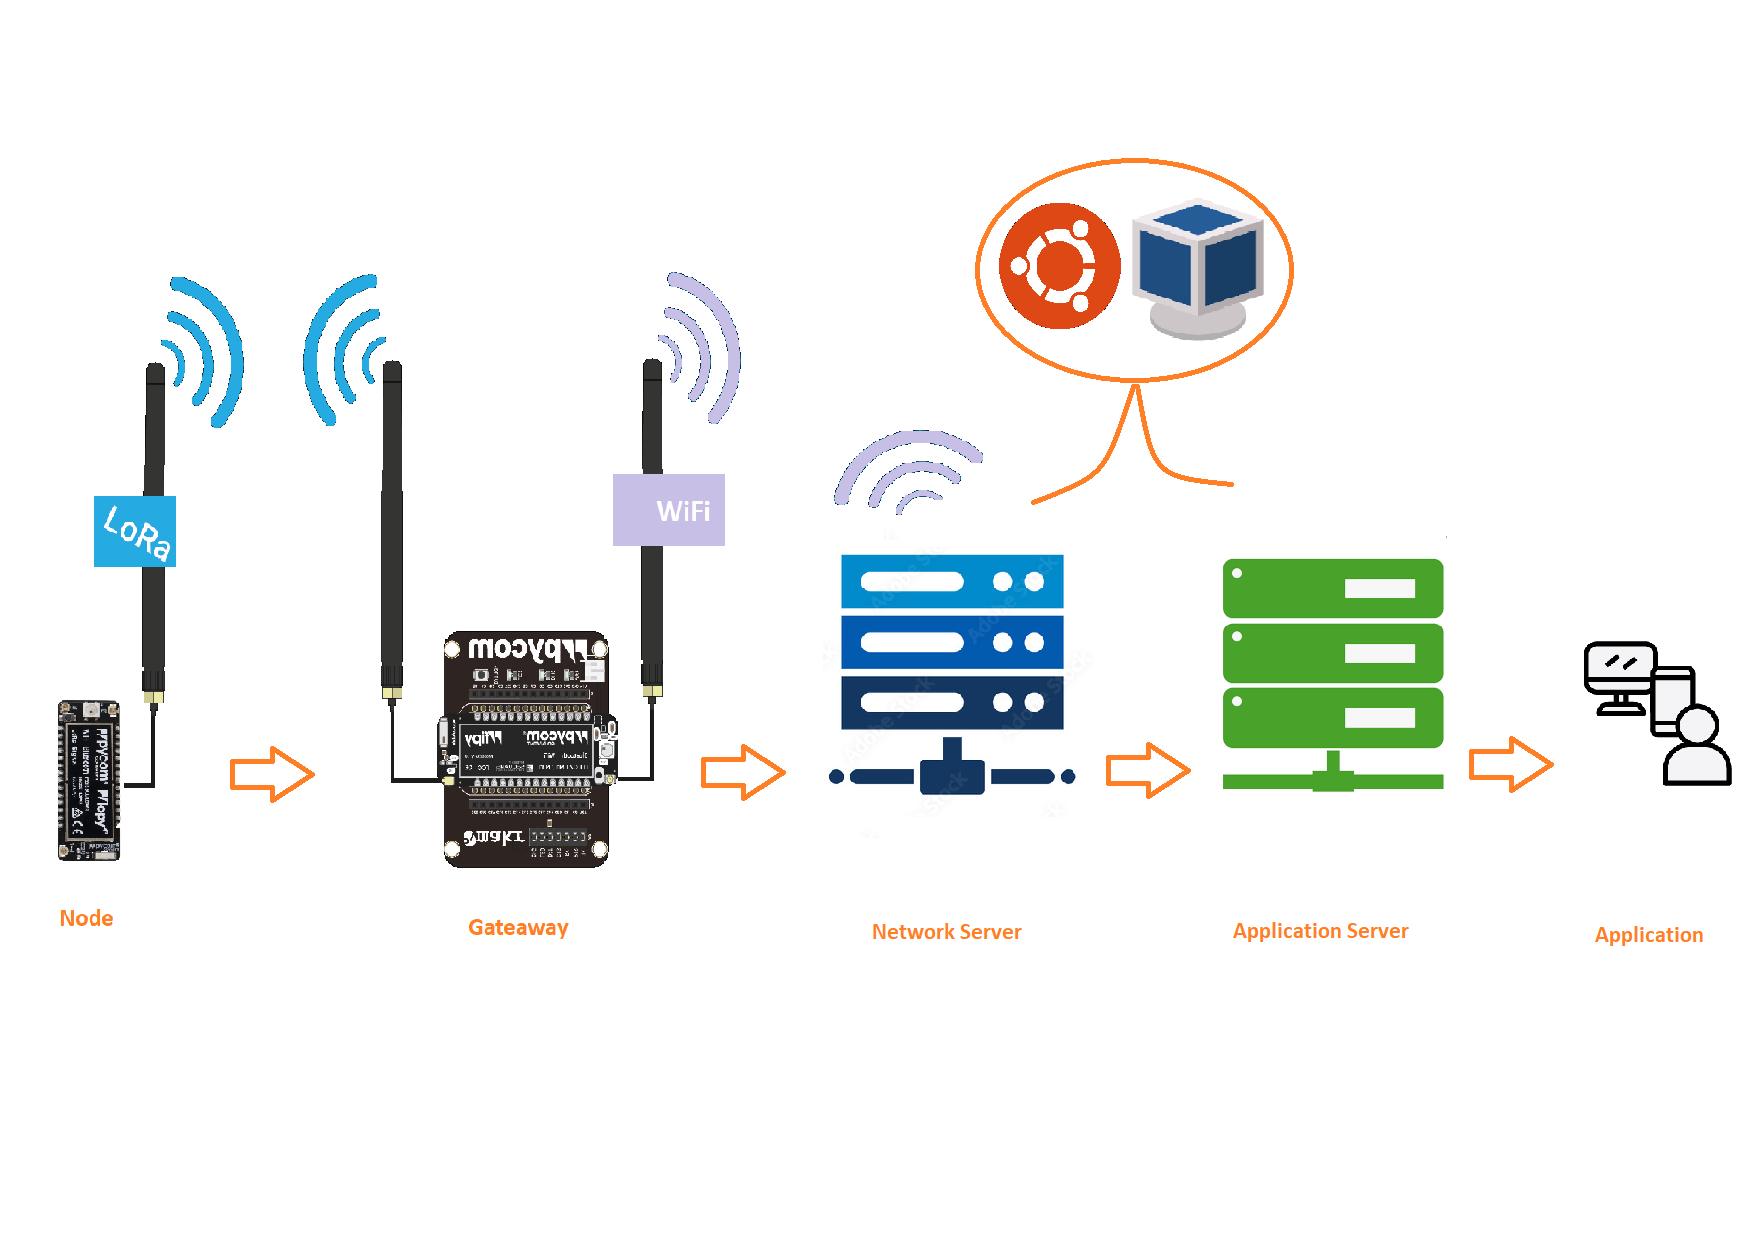
\includegraphics[scale=0.25]{figs/network.png}
	\caption{Network}\label{fig:network}
\end{figure}




 



